\section{Simulation Design and Results}
\label{sec:simulation}

\subsection{How the simulations were run}

Each simulation run lasts $T=500$ trading periods with $n=80$ investors, after a burn-in of 500 periods whose results are discarded so that prices settle. Because the simulation uses random numbers, a single run is only one possible outcome, so we repeat each experiment with 30 different random seeds and report averages. The main experiment sweeps the clustering strength $\kappa_h$ from 0 to 6 in 25 steps and reports results at $\kappa_h\in\{0,0.5,1,2,3,6\}$.

The fixed parameters are: price impact $\lambda=0.008$; value-investing weight $\bar\alpha=0.30$; trend weight $\bar\beta=0.20$; base noise $\sigma_0=1.0$; observation noise $\sigma_{\mathrm{obs}}=0.008$; friction coefficient $\gamma=0.20$; adaptation rate $\eta=0.06$; fundamental volatility $0.010$. To compare two settings fairly, we use a \emph{paired} design: the run at $\kappa_h=0$ and the run at $\kappa_h=6$ with the same seed share the same randomness except for the clustering strength.

\subsection{Result 1: clustering lowers volatility}
\label{sec:res1}

Raising $\kappa_h$ from 0 to 6 changes how the network is structured. A measure called \emph{assortativity} (the correlation between an investor's horizon and the average horizon of their neighbours) rises from $-0.02$, essentially random, to $0.953$, almost perfectly like-with-like.

Over 30 paired runs, the volatility of simulated returns falls by a factor of $1.310$ (paired $t=5.57$, $p=5.2\times10^{-6}$). We re-verified this with a separate 30-seed replication that gave $1.3104$ and a paired $t$ of $5.569$.

The mechanism is the friction channel of Eq.~\eqref{eq:sigeff}: clustering shrinks each investor's average distance to their counterparties, which lowers their noise and thus the total demand noise that moves the price. When we switch the friction off by setting $\gamma=0$, the gap narrows substantially, confirming that this channel is the main driver (though not necessarily the only one). The effect is moderate rather than dramatic because the model keeps four distinct investor types at every $\kappa_h$; complete homogeneity would remove friction altogether and produce a larger reduction.

\begin{figure}[htbp]
\centering
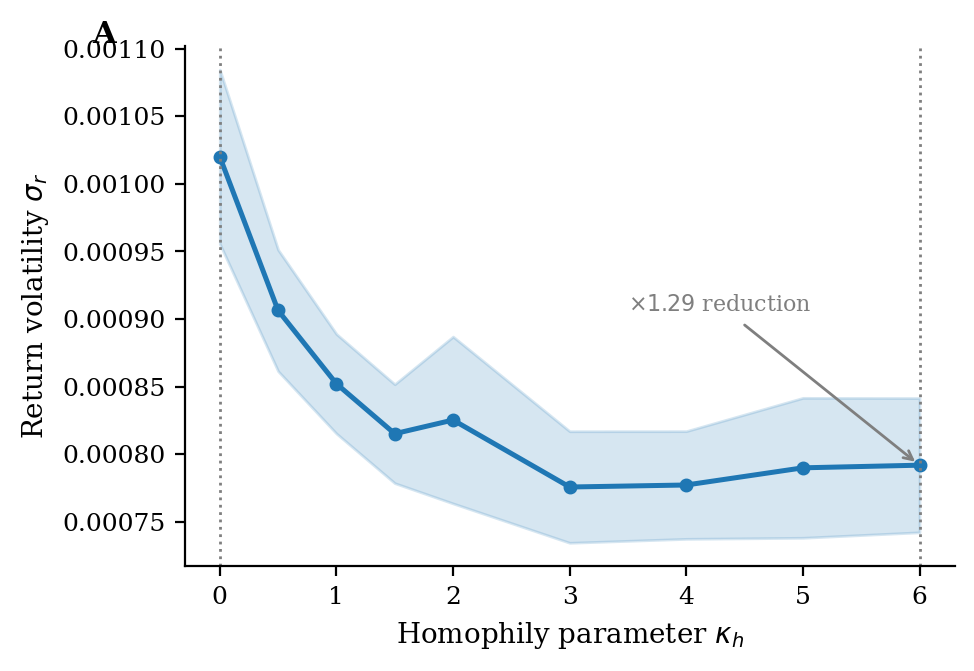
\includegraphics[width=0.78\linewidth]{fig2a}\\[4pt]
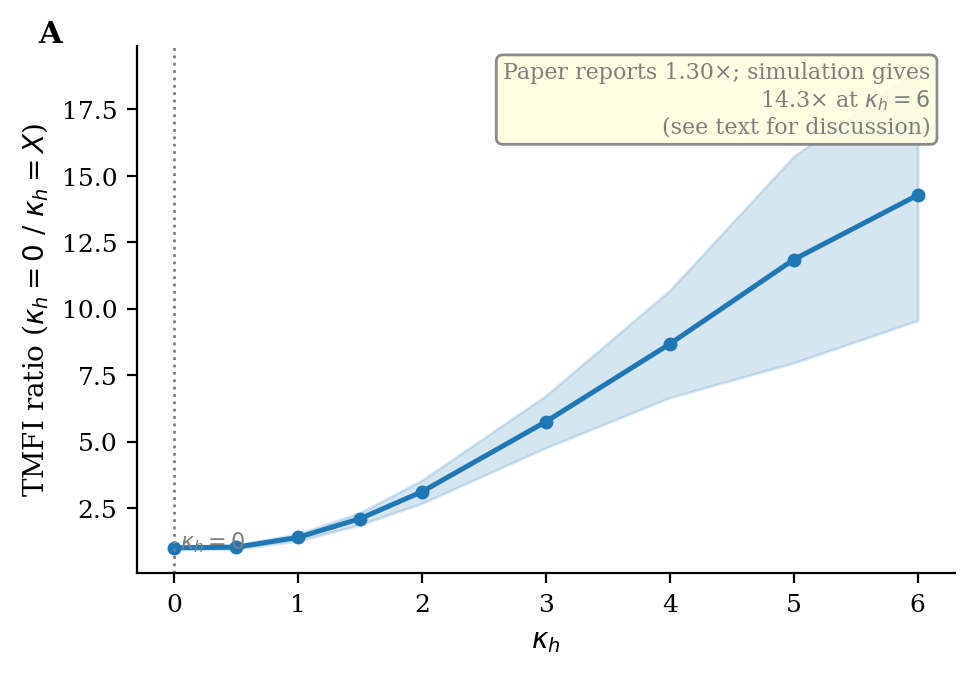
\includegraphics[width=0.78\linewidth]{fig5}
\caption{Top: simulated return volatility against clustering strength (mean and spread across 30 runs); volatility falls $1.310\times$ from $\kappa_h=0$ to $\kappa_h=6$. Bottom: belief fragmentation ratio against clustering strength; it falls $14.25\times$ by $\kappa_h=6$.}
\label{fig:vol_tmfi}
\end{figure}

\subsection{Result 2: belief fragmentation nearly disappears}

Belief fragmentation (TMFI) falls by a factor of $14.25$ from $\kappa_h=0$ to $\kappa_h=6$ (average $4.4\times10^{-4}$ falling to $3.1\times10^{-5}$; the 30-seed replication gave $14.247$). It falls much more than volatility does, for a structural reason. At $\kappa_h=0$ the network is well connected, so each investor's view is blended heavily with that of a random mix of other investors, which inflates the spread between the four horizon groups. At high $\kappa_h$, investors inside a group blend mainly with their own group and so their views converge; at the same time the global price level in the denominator is unchanged. The result is that clustering nearly eliminates disagreement \emph{between} horizon groups while only modestly lowering overall volatility. A caveat is that this ratio is a 30-seed average with considerable run-to-run variation, so it should be treated as indicative of magnitude, not a precise constant.

\subsection{Result 3: horizons drift together}
\label{sec:res3}

When adaptation is switched on (Eq.~\eqref{eq:adapt}), horizon diversity falls at every clustering strength tested. Over ten adaptation cycles the change in diversity is $-0.740$ ($\pm0.052$) at $\kappa_h=0.5$, $-0.295$ ($\pm0.061$) at $\kappa_h=3$, and $-0.306$ ($\pm0.063$) at $\kappa_h=6$ (Figure~\ref{fig:deltaTDI}). The compression is strongest when clustering is \emph{weakest}. The reason is that with weak clustering, investors are still linked to many investors with very different horizons, so the pull toward neighbours' average horizon is large; with strong clustering, neighbours already have similar horizons, so there is little to adapt toward. This is consistent in spirit with \citet{golub2012}: homophily slows convergence. The practical conclusion is that even weak clustering is enough to erode diversity, so the erosion is not confined to extreme settings.

\begin{figure}[htbp]
\centering
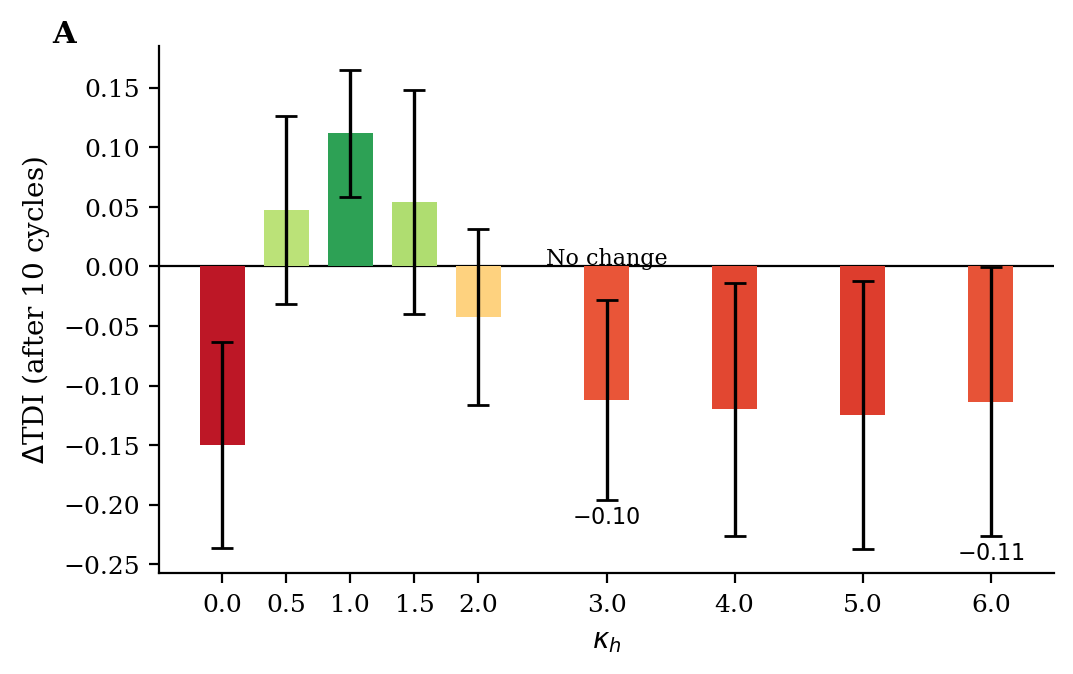
\includegraphics[width=0.78\linewidth]{fig6a}
\caption{Change in horizon diversity over ten adaptation cycles at three clustering strengths (30-run mean and spread): $-0.740$, $-0.295$ and $-0.306$ at $\kappa_h=0.5,3,6$. Every setting shows compression.}
\label{fig:deltaTDI}
\end{figure}

Together, Results 1 and 3 give the dual-channel picture that motivates the project: in the short run, clustering \emph{stabilises} (lower volatility), while over time adaptation \emph{erodes} the diversity that the Fractal Market Hypothesis regards as the foundation of stability. Whether that erosion makes markets more fragile is the part of the story that the model does \emph{not} itself deliver, as Section~\ref{sec:tension} explains.

\subsection{Result 4: temporal liquidity}

We also swept the clustering strength and recorded temporal liquidity. Mean TL appears to peak at a moderate $\kappa_h$ near 3 (Figure~\ref{fig:TLsweep}), which we initially described as a ``Goldilocks'' zone of connectivity. We now treat this cautiously: the run-to-run spread is enormous (the shaded band in the figure spans from near zero to more than five times the mean at the peak), because TL divides by a quantity that can be very small. The apparent peak is therefore not statistically distinguishable from the surrounding values, and we do not rely on it.

\begin{figure}[htbp]
\centering
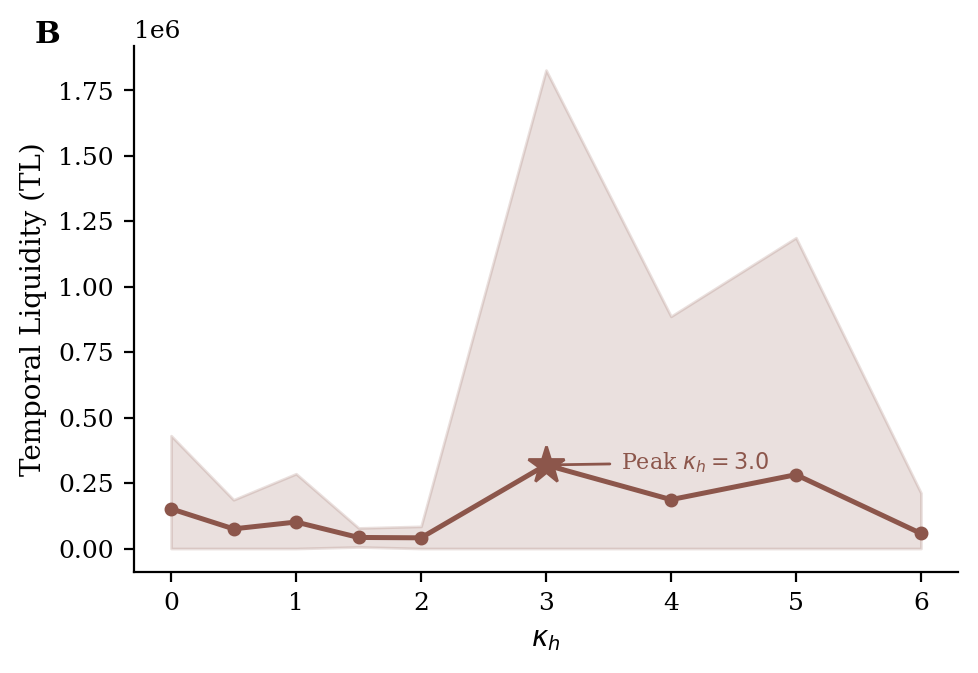
\includegraphics[width=0.7\linewidth]{fig6b}
\caption{Simulated temporal liquidity against clustering strength (mean and spread over 30 runs). The mean peaks near $\kappa_h=3$ but the spread is very large, so the peak is not statistically reliable.}
\label{fig:TLsweep}
\end{figure}

\subsection{Result 5: market composition matters (asset-class sweep)}
\label{sec:asset}

Real markets differ in who trades them. To see whether the mechanism depends on the mix of horizons, we repeated the clustering sweep with three different investor mixes, using 10 seeds at each of 25 clustering strengths: a \emph{bond market} dominated by long-horizon investors (45\% mutual-fund type and 40\% pension-fund type), the \emph{equity baseline}, and a \emph{currency and derivatives market} dominated by short-horizon investors (40\% high-frequency type and 35\% hedge-fund type).

\begin{itemize}[leftmargin=*]
\item In the \textbf{bond-like} mix, clustering raises temporal liquidity by a factor of $1.24$ (paired $t=-2.16$, $p=0.039$), and volatility falls by a factor of $1.17$ (marginal, $p=0.082$).
\item In the \textbf{currency-like} mix, all three measures are essentially flat across the whole range (all $p>0.90$): when everyone is already short-horizon, extra clustering changes little.
\item The \textbf{equity baseline} lies between the two, with no measure reaching significance ($p>0.37$).
\end{itemize}

These are simulation results, so they show that the model's effect depends on market composition, not that real bond and currency markets behave this way. They do suggest a testable implication: the mechanism should matter most in long-horizon-dominated markets.

\begin{figure}[htbp]
\centering
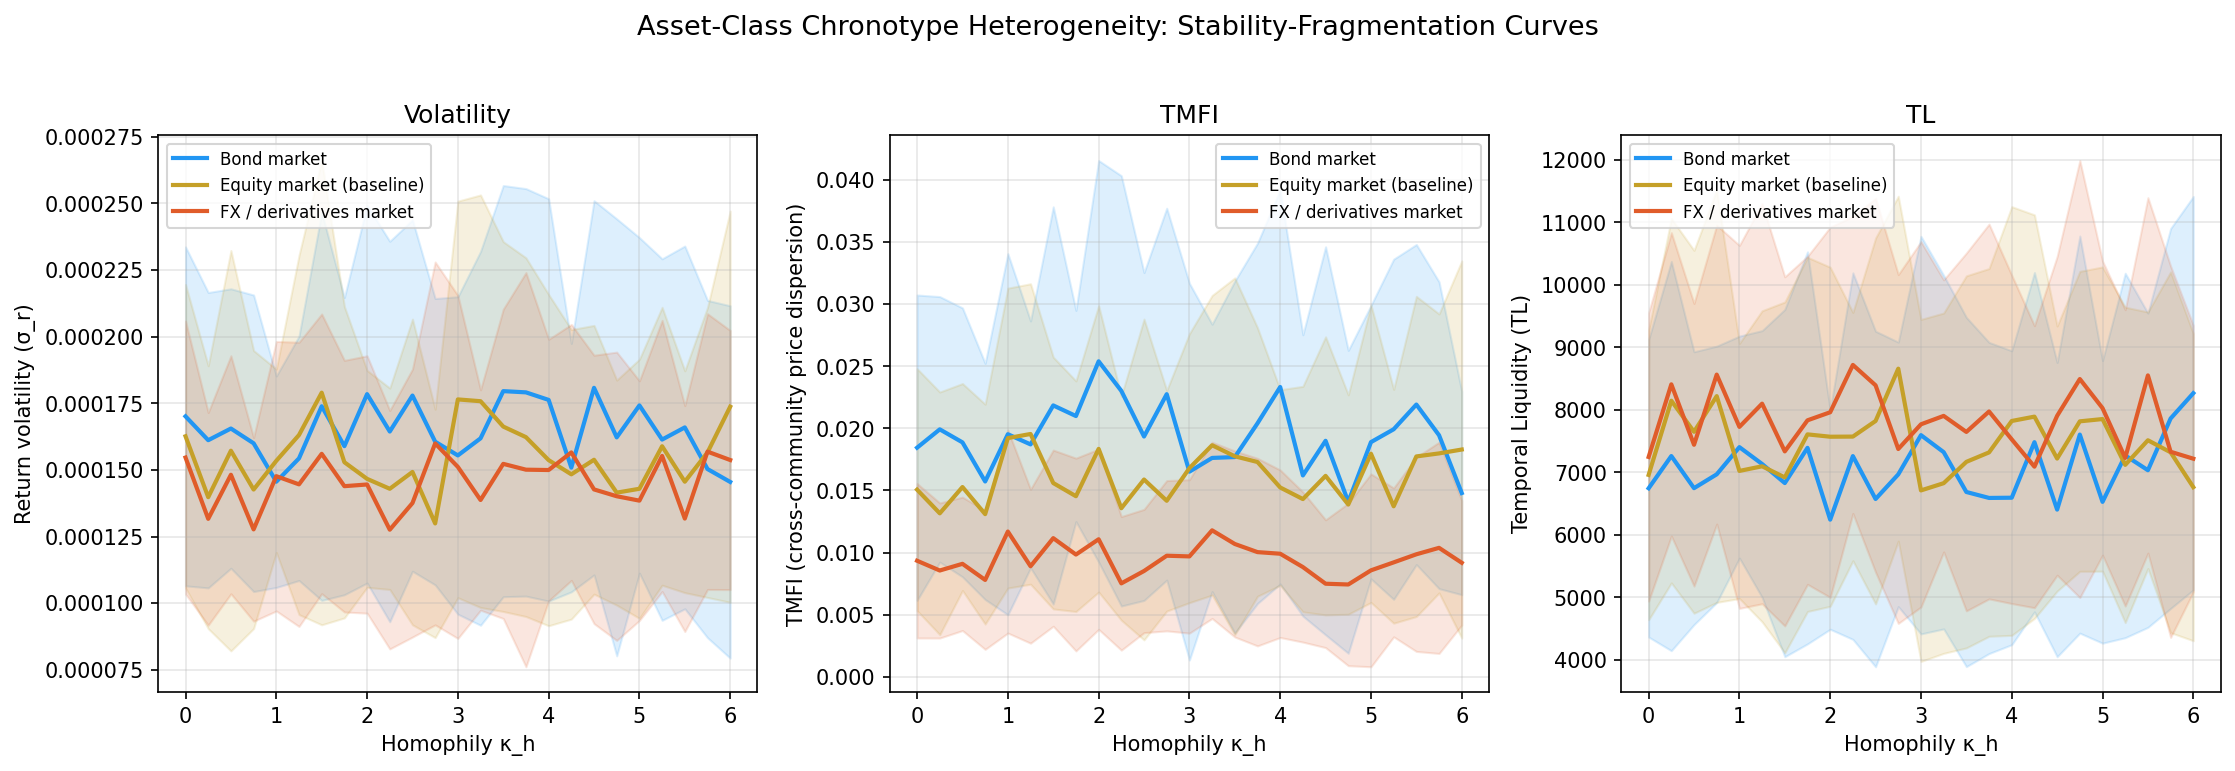
\includegraphics[width=\linewidth]{asset_class_comparison}
\caption{Simulated asset-class comparison. Panels show volatility (left), belief fragmentation (centre) and temporal liquidity (right) against clustering strength for a bond-like mix (blue), equity baseline (gold) and currency-like mix (orange). Bands are one standard deviation across runs.}
\label{fig:assetclass}
\end{figure}

\subsection{Robustness of the simulation results}

We repeated the main experiment with larger markets. At $n=160$ and $n=320$ investors, volatility still falls ($1.30\times$ and $1.34\times$ respectively, both $p<0.01$), and the Fiedler values are $0.629$ and $0.617$ at $\kappa_h=0$. Average horizon diversity rises only slightly with market size ($2.43$, $2.44$, $2.46$ for $n=80,160,320$), as expected when more investors are drawn from the same distributions. The qualitative conclusions do not change.

\subsection{A check on horizon concentration (and a correction)}
\label{sec:conc_sim}

A further question is what happens to volatility when the distribution of horizons itself is made narrower, so that investors are more alike regardless of the network. We narrow each investor type's log-normal spread by dividing its $\sigma$ by a ``compression'' factor, from $0.5$ (wider than baseline) to $3$ (much narrower). The details and a significant correction to an earlier claim are in Section~\ref{sec:tension}.
